\section[Heat Capacity Models I — Boltzmann and Einstein]{\hyperlink{toc}{Heat Capacity Models I — Boltzmann and Einstein}}


Chapter 2 covers the Specific Heat of Solids

Recall:
\begin{itemize}
    \item Heat capacity of material is how much energy (heat) you need to add to change the temp (by 1K).
    \begin{equation}
        C = \frac{d \left<E \right>}{dT}
    \end{equation}

    \item Solids are incompressebile so $C_v \simeq C_p $
    \item ``specific heat" and ``heat capacity" are used interchangeably
    \item strictly we are speaking about molar heat capacity (per mol of material) with units of $\left[ J/\text{mol}\cdot K\right]$
    \item 
    \[ 1 \, \text{mol} = N_A = 6.022 \times 10^{23}\]

\end{itemize}

Why do we care?

\begin{itemize}
    \item gives us info about thermally excited states and so we can look for phase transitions 
    \item largest factor in specific heat is atomic vibrations
\end{itemize}

Heat capacity of an ideal monoatomic gas at constant volume (3-D)
\begin{itemize}
    \item Equipartiion theorem: each quadratic degree of freedom in the energy contributes $\frac{1}{2} k_BT$ to $\left< E\right>$
    \item Ideal Gas only has kinetic energy with x, y, and z components so we get
    \begin{equation}
        \left<E\right> = \frac{3}{2} k_B T
    \end{equation}
    per atom
    \begin{equation}
        \left<E\right> = \frac{3}{2} R T
    \end{equation}
    per mol
    \begin{equation}
        C = \frac{d\left< E \right>}{dT} = \frac{3}{2} R
    \end{equation}

    \item Note that:
    \[R = N_A \cdot k_B = 8.314 J/\text{mol}\,K\]
\end{itemize}

Experimental observations from 1820-1910
\begin{itemize}
    \item Dulong-Petit Law:
    \begin{equation}
        C = 3 k_B 
    \end{equation}
    per atom (or $C=3R$ per mol)
    \item Boltzmann made classical statistical model that explained the Dulong-Petit result
    \begin{itemize}
        \item It treated each atom as a \textbf{simple harmonic oscillator} 
        \item each of which were held in place in each direction by a spring vibrating t a frequency, $\omega$.

        \begin{equation}
            \hat{H} = \frac{\hat{p}^2}{2m} + \frac{k\hat{x}^2}{2}
        \end{equation}

        where $\omega = \sqrt{\frac{k}{m}}$ which you will show on HW1 that it gives $C=3R$

        \item But this still does not explain diamond or any solid significantly below room temperature
    \end{itemize}

    \item Thermodynamics refresher

    \begin{itemize}
        \item The probability of finding a system, S, that is in thermal equilibrium with a reservoir, R, at some temperature, T, in a given energy state, $E_i$, 
        \begin{center}
        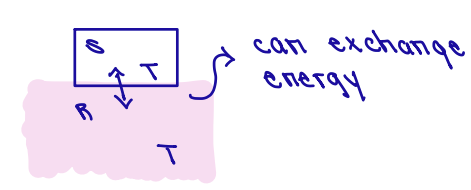
\includegraphics[width = 0.25\textwidth]{Images/Lecture2-thermo.png}
        \end{center}
        
        is given by 

        \[
        \mathbb{P}(E_i) \propto \mathrm{e}^{-\beta E_i}
        \]

        where $\beta = \frac{1}{k_B T}$ with units of $\left[ \frac{1}{\text{energy}}\right]$

        Note that the exponential term is the Boltzmann distribution

        \item We can use the \textbf{partition function (Z)} to normalize our probabilities.

        i.e. so that we get $\sum_i \mathbb{P} (E_i) = 1$

        \[ \mathbb{P} (E_i) = \frac{\mathrm{e}^{-\beta E_i}}{\mathrm{e}^{-\beta E_1} + \mathrm{e}^{-\beta E_2} + \dots } = \frac{\mathrm{e}^{-\beta E_i}}{Z}\]

        where $Z = \sum_i \mathrm{e}^{-\beta E_i}$

        \item The \textbf{expecation value (or thermal average)} for a given quantity is the sum of the possible values weighted by their normalized probabilities.

        \[ \angles{x} = \sum_i x_i \Prob (E_i) = \sum_i x_i \paren*{\frac{\e^{-\beta E_i}}{Z}} = \recip{Z} \sum_i x_i \e^{-\beta E_i} \]

        where $ Z = \sum_i \e^{-\beta E_i} $

        \item Taking the \textbf{derivative of the partition function with respect to $\beta$} we uncover a useful trick.

        \[ \dv{Z}{\beta} = \sum_i \paren*{-E_i } \, \e^{-\beta E_i} \]

        Divide by $-Z$ and we get 

        \[ \frac{-1}{Z} \dv{Z}{\beta} = \recip{Z} \sum E_i \e^{-\beta E_i} = \angles{E}\]

        Thus we get the equation that relates the average internal energy to the partition function.

        \[ \angles{E} = \frac{-1}{Z} \dv{Z}{\beta}\]

        which is useful because we want to calculate $C = \dv{\angles{E}}{T}$

        \item \textbf{Bose-Einstein} and \textbf{Fermi-Dirac Statistics} to describe the energy distribution of quantum particles 

        \begin{itemize}
            \item BE: photons, cooperes pairs, He$^4$, atomic vibrations (phonons)
            \begin{itemize}
                \item The Bose occupation factor $n_B$ gives the number of bosonic particles occupying a given energy state at a given temperature.

                As $T \xrightarrow{} 0$, all particles occupy the ground state.
        
                \begin{center}
                    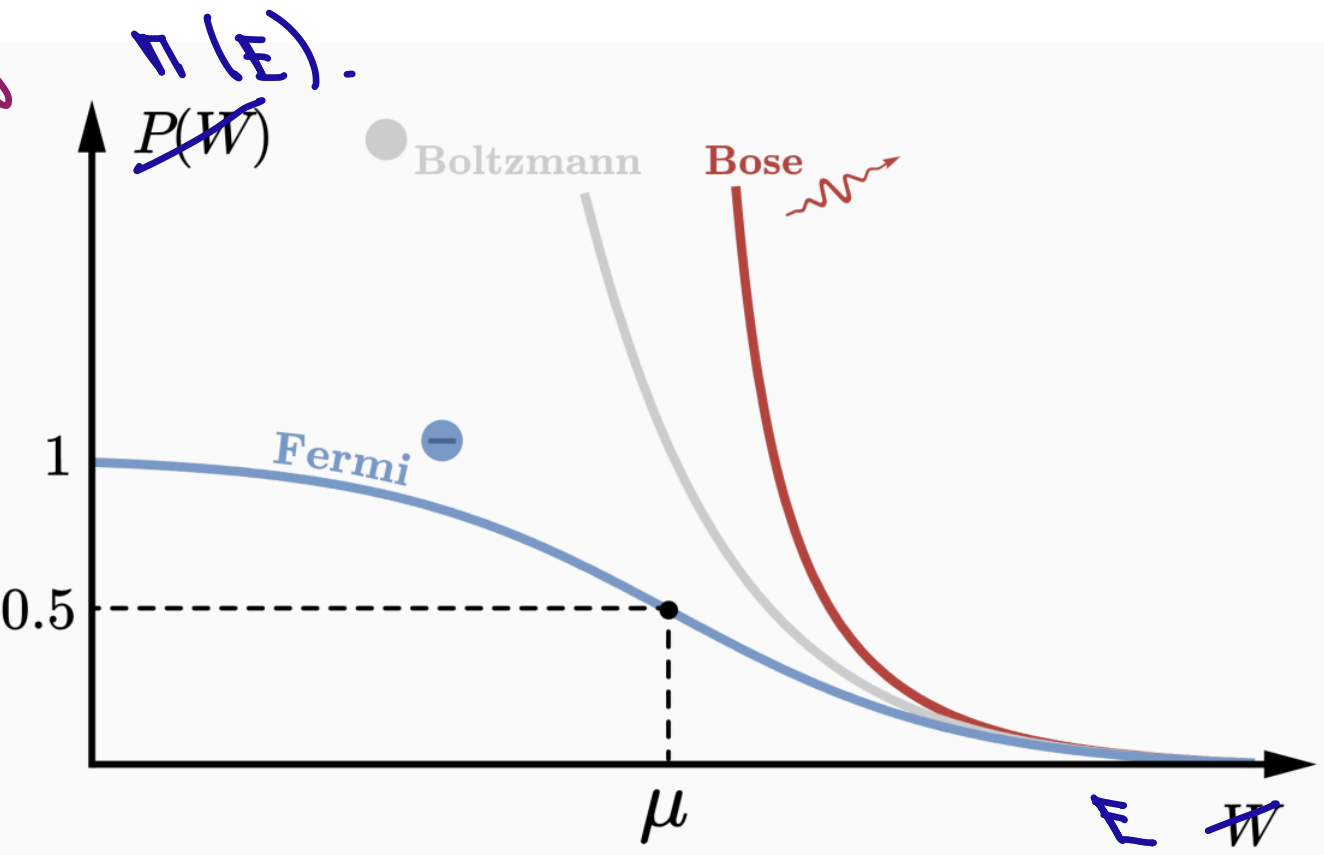
\includegraphics[width = 0.4 \textwidth]{Images/ground-state-distribution-bose-fermi.png}
                \end{center}
        
                \[ n_B = \recip{\e^{(E-\mu) \beta} -1}\]
        
                \vspace{1px}
                
                \item where in the high T limit looks identical to Boltzmann distribution.
        
                \item as $T \rightarrow 0$, $\beta \rightarrow$ and only the lowest E state ($E \approx \mu$) is occupied
        
                \item and $\mu$ is the chemical potential (energy cost to add a particle to the system
            \end{itemize}
            \item FD: electrons, other leptons, He$^3$
            \begin{itemize}
                \item The Fermi factor $n_F$ gives the number of fermionic particles occupying a given energy state at a given temperature where each state can only be single occupied due to the Pauli exclusion principle.

                \[ n_F = \recip{\e^{(E-\mu )\beta} + 1}\]
                \item also looks identical to the Boltzmann distribution in the high T limit
            \end{itemize}
        \end{itemize}
    \end{itemize}

\end{itemize}




